%----------------------------------------------------------------------------------------
%	PACKAGES AND OTHER DOCUMENT CONFIGURATIONS
%----------------------------------------------------------------------------------------

\documentclass[11pt]{article}
%\input{mydef.tex}
\usepackage{fancyhdr} % Required for custom headers
\usepackage{lastpage} % Required to determine the last page for the footer
\usepackage{extramarks} % Required for headers and footers
\usepackage[usenames,dvipsnames]{color} % Required for custom colors
\usepackage{graphicx} % Required to insert images
\usepackage{listings} % Required for insertion of code
\usepackage{courier} % Required for the courier font
\usepackage{amssymb,amsmath}
\usepackage{amsfonts}
\usepackage{mathtools}
%\usepackage{subfigure}
\usepackage{enumitem}
\usepackage{bm}
\usepackage{url}
\usepackage[stable]{footmisc}
\usepackage{booktabs}
\usepackage[square]{natbib}
\usepackage{indentfirst}
%\usepackage[colorlinks, linkcolor=red, anchorcolor=purple, citecolor=blue]{hyperref}
\usepackage{hyperref}
\usepackage{subcaption}
\usepackage{graphicx}

\usepackage{multicol}
\setlength{\columnsep}{1cm}

% Margins
\topmargin=-0.45in
\evensidemargin=0in
\oddsidemargin=0in
\textwidth=6.5in
\textheight=9.0in
\headsep=0.25in
\setlength{\headheight}{13.6pt}
\linespread{1.1} % Line spacing

% Set up the header and footer
\pagestyle{fancy}
\lhead{CS 57800} % Top left header
\chead{}
\rhead{Homework} % Top right header
\lfoot{} % Bottom left footer
\cfoot{} % Bottom center footer
\rfoot{Page\ \thepage\ of\ \protect\pageref{LastPage}} % Bottom right footer
\renewcommand\headrulewidth{0.4pt} % Size of the header rule
\renewcommand\footrulewidth{0.4pt} % Size of the footer rule

\renewcommand*{\thefootnote}{\fnsymbol{footnote}}

\setlength{\parskip}{.2\baselineskip}
%\setlength\parindent{0pt} % Removes all indentation from paragraphs

\title{
\textbf{CS57800 Statistical Machine Learning} \\ \textsc{Homework 2} \\
\normalsize\vspace{0.1in}
}

\author{
	\textbf{Ting Zhang} \\
	School of Industrial Engineering\\
	\texttt{zhan1013@purdue.edu}
}

\date{\today}
%----------------------------------------------------------------------------------------

\begin{document}

\maketitle
%\thispagestyle{empty}

\section{Foundations}
\begin{itemize}
\item[1.]
(1) Boolean function \\
\(f(x_1,x_2,x_3,x_4)=\neg[(x_1\wedge \neg x_2\wedge \neg x_3\wedge\neg x_4)\vee
                     (\neg x_1\wedge  x_2\wedge \neg x_3\wedge\neg x_4)\vee
										 (\neg x_1\wedge \neg x_2\wedge  x_3\wedge\neg x_4)\vee
										 (\neg x_1\wedge \neg x_2\wedge \neg x_3\wedge x_4)\vee
										 (\neg x_1\wedge \neg x_2\wedge \neg x_3\wedge \neg x_4)] \) \\
(2) Linear function\\
\(f(x_1,x_2,x_3,x_4)=1 \quad \mathrm{if} \quad x_1+x_2+x_3+x_4 \geq 2\)
\item[2.]
\(size(CON_B)=2^n \)
\item[3.]
Since \(\beta_n = \beta_o+y_i u_i \), then
\begin{align*}
\|\beta_n-\beta^*\|^2 &=\|\beta_o+y_i u_i-\beta^*\|^2 \\
                      &=(\beta_o-\beta^*)^2+2y_i u_i(\beta_o-\beta^*)+(y_i u_i)^2 \\
											&=(\beta_o-\beta^*)^2+2(\beta_o y_i u_i-\beta^*y_i u_i)+(y_i u_i)^2
\end{align*}
Since \(u_i={x_i}^*/\|{x_i}^*\|\), then \(u_i=\pm 1\). Also, because \(u_i\) is a misclassified example, then \(y_i \cdot (\beta_o u_i)<0\). Because \(\beta^*\) is the final separating parameter vector, we will have \(y_i \cdot (\beta^* u_i) \geq 1\) (Proved later). Substitute these values into the above equation, we will have:
\begin{align*}
\|\beta_n-\beta^*\|^2 & \leq \|\beta_o-\beta^*\|^2+2(0-1)+1 \\
                      &=\|\beta_o-\beta^*\|^2-1 
\end{align*}
To prove \(y_i \cdot (\beta^* u_i) \geq 1\): Since we can finally separate these data, here we assume \(\beta\) is the separating hyperplane, then we have \(y_i \cdot (\beta u_i)>0\) for every \(u_i\). Let's assume \(m\) is the minimum value of this product, then we can have \(y_i \cdot (\beta x_i) \geq m>0\). Move \(m\) to the left side of the inequality, we will have \(y_i \cdot (\beta/m x_i) \geq 1\). Since  \(\beta^*\) is the final separating parameter vector, we have    \(\beta^*=\beta/m\), such that \(y_i \cdot (\beta^* u_i) \geq 1\).
\item[4.]
Assume there are \(n\) Boolean varaibles, defined as \(x_1,x_2,x_3,...,x_n\). To learn the conjunction function consistituted with these variables, we denoted the learnt function as \(f(x)\).\\
First, we initialize the function as: \(f(x)=x_1 \wedge x_2 \wedge ... \quad x_n \wedge \neg x_1 \wedge \neg x_2 \wedge ... \neg x_n\)\\
Then, we start learning this function by passing examples one by one. We can observe that this function can only make mistakes on positive examples, therefore, we can learn this function with positive examples.\\
if there is an mistake, eliminate all items that equals 0 in the example from the learnt function \(f(x)\). The  item here refers to one item in \(f(x)\). For example, \(x_i\) and \(\neg x_i\) are both iterms of the function. Then in the first example, half of the items in \(f(x)\) will be eliminated since the initial \(f(x)\) contains both the variable and the negation of the variable. If \(x_i=1\), then \(\neg x_i\) must be 0. Therefore, you can only have one of these two left after the first example, which means half of the items were eliminated.\\
After the first positive mistake, when it comes another positive mistake, the items equal \(0\) will be eliminated. This procedure continues until no more mistakes are made. This is a mistake bound algorithm, since for each mistake it made, at least one item will be eliminated. After the first positive example, there are \(n\) items left, and for these \(n\) items, there are at most \(n\) mistakes. Therefore, this algorithm is bounded for \(n+1\) mistakes.
\item[5.]
(1) Both classifiers will converge since the data is linearly separable. However, the one with sorted dataset may converge slower than the one with randomized order.
(2) The training error of the first classifier would be 0\%. And the training error for the second classifier would be 0\% since the data is linearly separable.
\item[6.]
Proof.
\begin{align*}
\|\sum_{i\in N} y_i x_i\| & = \|\sum_{i\in N} (w_{i+1}-w_i)\| \\
                          & = \| (w_{i+1}-w_i)+(w_i-w_{i-1})+(w_{i-1}-w_{i-2})+...+(w_1-w_0) \| \\
													& = \|w_{i+1}\| \\
													& = \sqrt{(\|w_{i+1}\|^2-\|w_i\|^2)+(\|w_i\|^2-\|w_{i-1}\|^2)+...+(w_1^2-w_0^2)} \\
													& = \sqrt{\sum_{i\in N} (\|w_{i+1}\|^2-\|w_i\|^2)} \\
													& = \sqrt{\sum_{i\in N} (\|w_i+y_i x_i\|^2-\|w_i\|^2)} \\
													& = \sqrt{\sum_{i\in N} (\|w_i\|^2+2y_i w_i x_i+\|y_i x_i\|^2-\|w_i\|^2)} \\
													& = \sqrt{\sum_{i\in N} (2y_i w_i x_i+\|x_i\|^2)}
\end{align*}
Since these are the examples when Peceptron makes a mistake, therefore, \(y_i w_i x_i\leq 0\). So,
\begin{align*}
\|\sum_{i\in N} y_i x_i\| & \leq \sqrt{\sum_{i\in N} \|x_i\|^2}
\end{align*}
\end{itemize}


\section{Programming Report}
In this section, Perceptron and Winnow algorithm were implemented to predict positive or negative sentiment from single snippet movie review. For both algorithms, they follow the same procedure. First, features were extracted in three different representations, including unigram, bigram and both unigram and bigram. Then, the weights for each feature in the feature set were trained following each algorithm. At last, the sentiment can be predicted using the trained weights. Detailed explanation is presented in the following sections.
\subsection{Feature Extraction}
In this task, three representations of features were extracted and experimented with: 1) unigram, 2) bigram and 3) both unigram and bigram.
\begin{itemize}
\item[1)] Unigram: Each single word in the movie reviews were extracted as a feature.
\item[2)] Bigram: Two consecutive words in a snippet were extracted as one feature.
\item[3)] Use Both: The combination of both unigram features and bigram features.
\end{itemize}
In all these representations, the presense of a feature (one word or group of two words) is denoted as 1, therefore, a single snippet can be represented as a series of 1s and 0s.
\subsection{Perceptron and Winnow Algorithm}
Both of these onling learning algorithms learns on mistakes. To be specific, the weights for each active feature will be updated if the prediction is wrong in the input snippet.
\begin{itemize}
\item[1)] Perceptron: Initialize all weights,\(w\), and the bias term \(b\) to 0. And the weights for each active feature and bias term will be updated following this equation:
\begin{align*}
&w_d = w_d + yx_d \\
&b = b + y
\end{align*}
where \(d\) is the index for each feature, and \(y\) is the label for this input snippet.

After going through all the input snippets for a certain number of iterations, we should get fewer and fewer errors. This number of iterations is considered as a hyper-parameter that will be tuned using the validation set. The optimal number of iteration will be selected and the weights and bias term updated after this number of iteration will be used in the testing set. To predict the label for each snippet, perceptron simply following this equation:
\begin{align*}
a = \sum_{d=1}^{D}w_dx_d + b
\end{align*}
The sign of \(a\) would be the predicted label.
\item[2)] Winnow: Different from perceptron, winnow initialize all weights \(w\) to 1, and a fixed value \(\theta\) to the number of features \(n\). To update the weights for each feature, the equation depends on how the mistake is made. If the mistake is on a postive example, then the weights of active features will be doubled. If the mistake is on a negative example, the weights for active features will be halved, which can be represented in the following equations. 
\begin{align*}
\mathrm{if}  \quad  f(x)=1 \text, w_i = 2w_i  \quad (\mathrm{if} \quad x_i=1)\\
\mathrm{if} \quad f(x)=-1, w_i = w_i/2  \quad (\mathrm{if} \quad x_i=1)
\end{align*}
The same as perceptron, an optimal weights will be obtained by tuing the maximum number of iterations on validation set. To predict the label of on snippet, we can apply the following equations:
\begin{align*}
\sum_{d=1}^{D}w_dx_d
\end{align*}
If the summation is less than theta, then the predicted label would be -1; otherwise, it would be 1.
\end{itemize} 
\subsection{Experiment and Results}
Here, the results for tuning the hyper-parameter, maximum number of iterations, for all the feature set and onling learning algorithms are presented. Figure \ref{fig:1} shows the results for perceptron with (a)Unigram, (b)Bigram and (c)Both feature set. Figure \ref{fig:2} shows the results for winnow algorithm.
\subsubsection{Perceptron algorithm}
For unigram feature set, perceptron converged at iteration 58 for the training set and reached it's highest accuracy, 72.5\%,  for validation set at iteration 40. For bigram feature set, perceptron didn't converge for the training set until iteration 100 with accuracy of 99.9\%. And the accuracy for validation set reached its highest on iteration10 for 62.7\%. For the one with both unigram and bigram feature set, perceptron converged quickly at iteration 15 for the training set, with the highest valiation accuracy of 71.8\% at iteration 5.

The testing set was then tested with weights after 40 iterations for unigram feature set, 10 iterations for bigram feature set and 5 iterations for both feature set. The accuracy of these feature set are: 71.2\%, 63.5\% and 73.1\%.
\begin{figure}
\begin{subfigure}{0.31\textwidth}
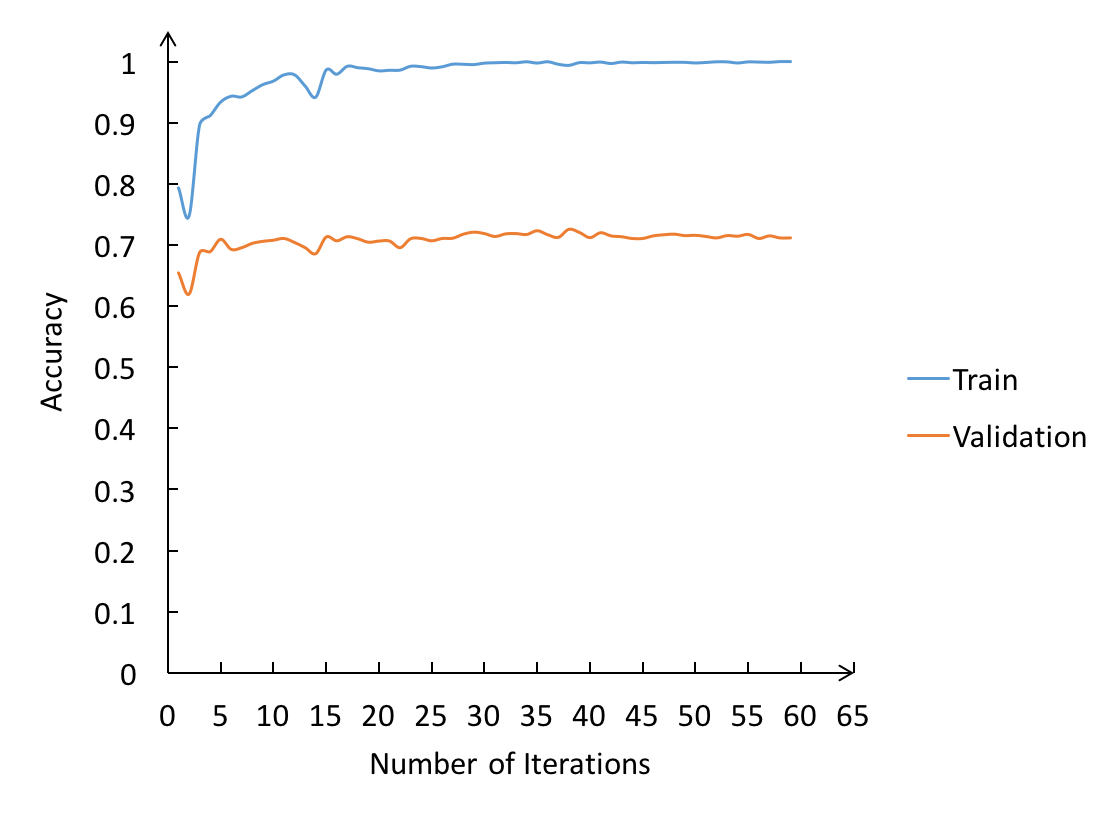
\includegraphics[width=\linewidth]{perceptron_unigram.png}
\caption{Unigram} \label{fig:1a}
\end{subfigure}
\hspace*{\fill} % separation between the subfigures
\begin{subfigure}{0.31\textwidth}
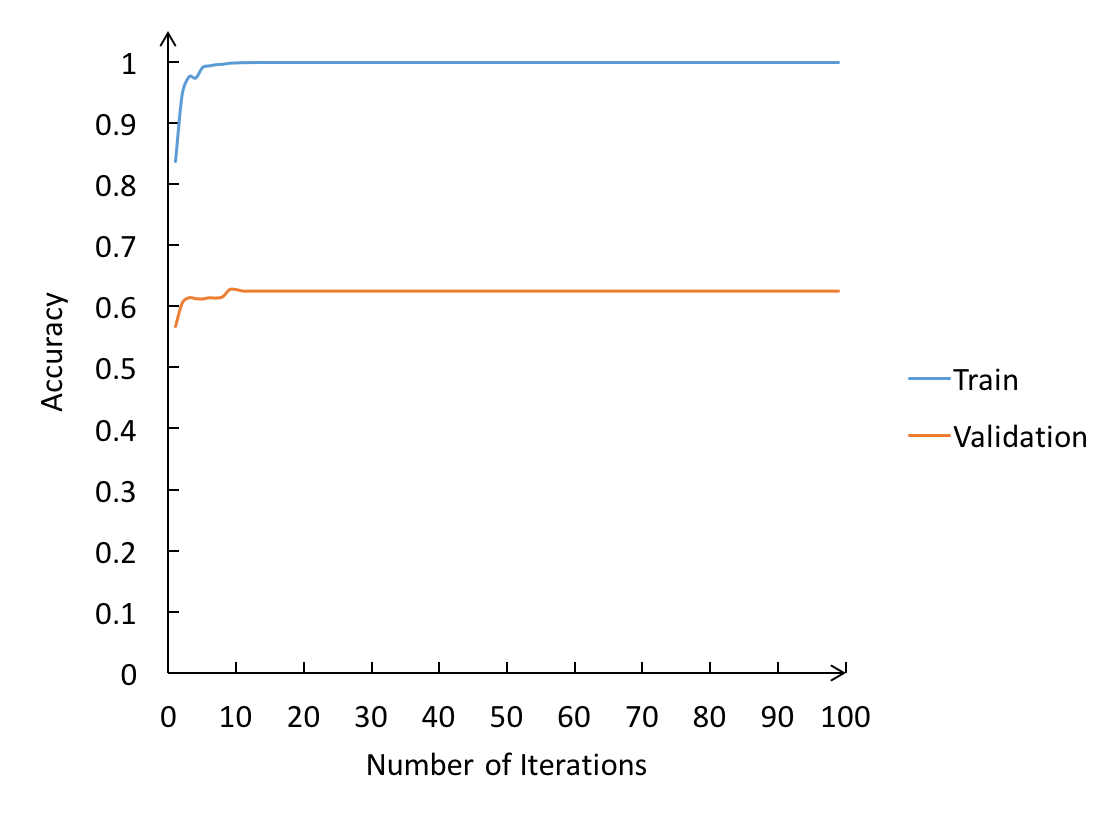
\includegraphics[width=\linewidth]{perceptron_bigram.png}
\caption{Bigram} \label{fig:1b}
\end{subfigure}
\hspace*{\fill} % separation between the subfigures
\begin{subfigure}{0.31\textwidth}
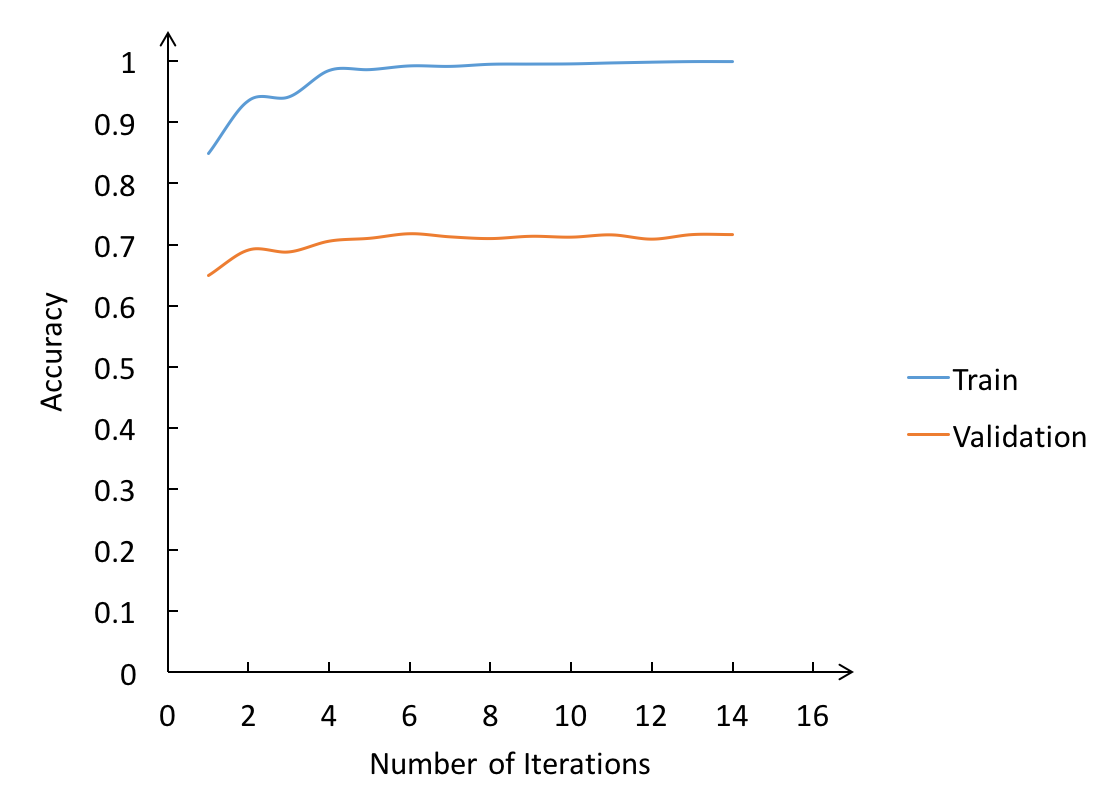
\includegraphics[width=\linewidth]{perceptron_both.png}
\caption{Both} \label{fig:1c}
\end{subfigure}
\caption{Results for Perceptron Algorithm} \label{fig:1}
\end{figure}
\subsubsection{Winnow algorithm}
For the winnow algorithm, no feature set actually converged after 100 iterations. Unigram feature set reached its highest accuracy of 93.9\% at iteration 66 for the t raining set. For the validation set, It reached its highest accuracy of 66.9\% at iteration 51. For the bigram feature, the accrucy of training set goes up to 99.9\% and reached the highest for validation set at iteration 25 of 60.1\%. For the one using both unigram and bigram feature set, the accuracy of trainning set reached 99.9\% at iteration 67. And the accuracy for validation set is 64.1\% at iteration 9.

The testing set was then tested with weights after 51 iterations for unigram feature set, 25 iterations for bigram feature set and 9 iterations for both feature set. The accuracy of these feature set are: 65.2\%, 62.2\% and 66.8\%.

\begin{figure}
\begin{subfigure}{0.31\textwidth}
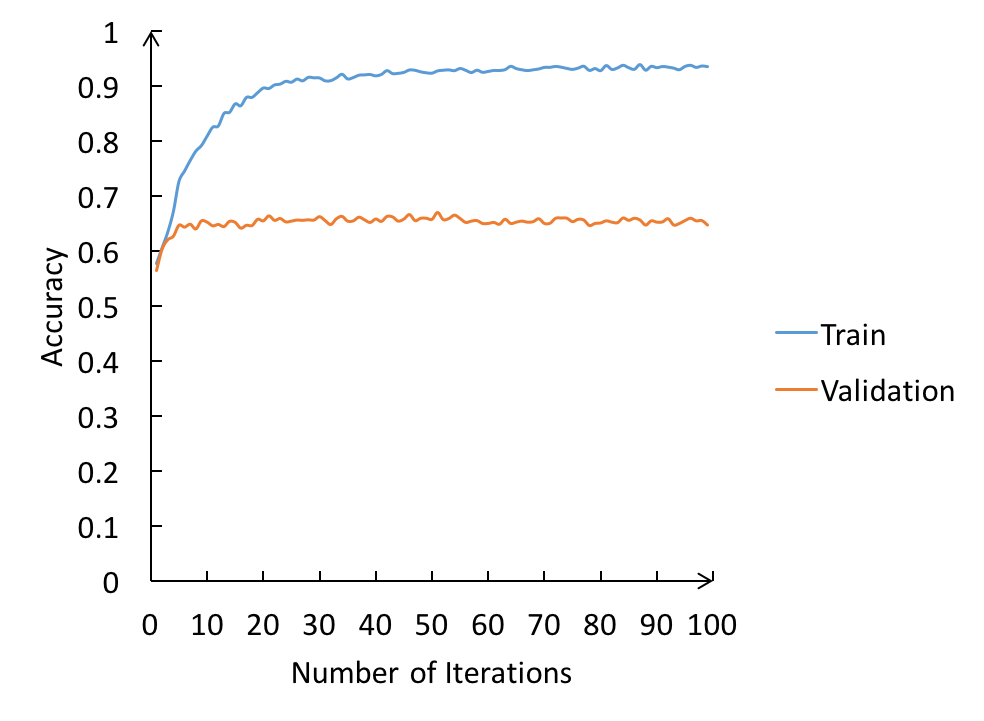
\includegraphics[width=\linewidth]{winnow_unigram.png}
\caption{Unigram} \label{fig:2a}
\end{subfigure}
\hspace*{\fill} % separation between the subfigures
\begin{subfigure}{0.31\textwidth}
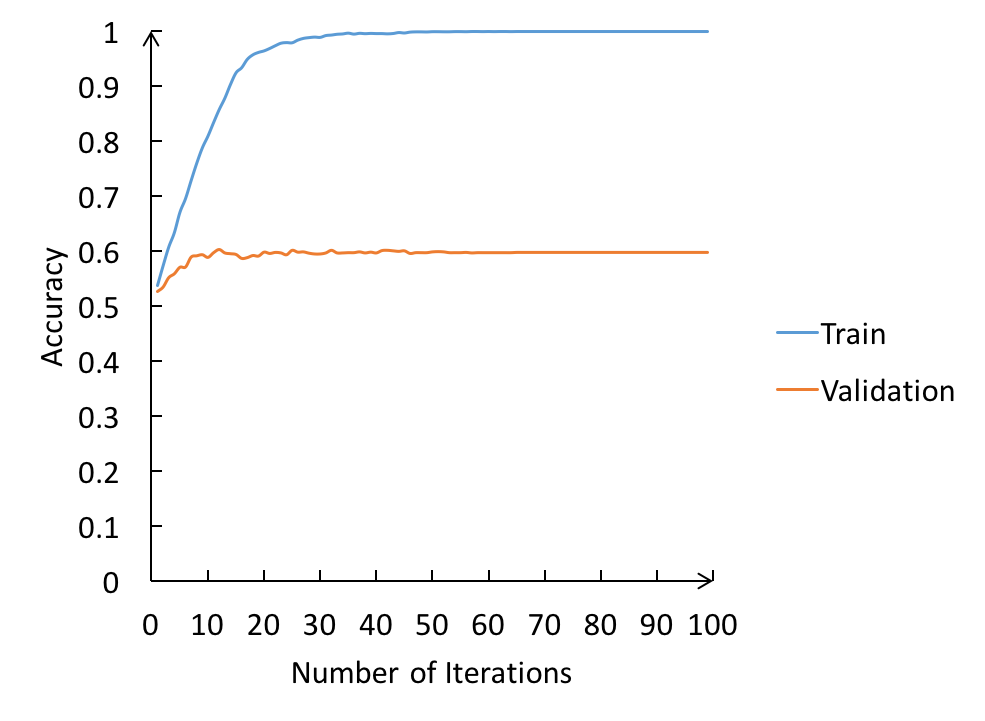
\includegraphics[width=\linewidth]{winnow_bigram.png}
\caption{Bigram} \label{fig:2b}
\end{subfigure}
\hspace*{\fill} % separation between the subfigures
\begin{subfigure}{0.31\textwidth}
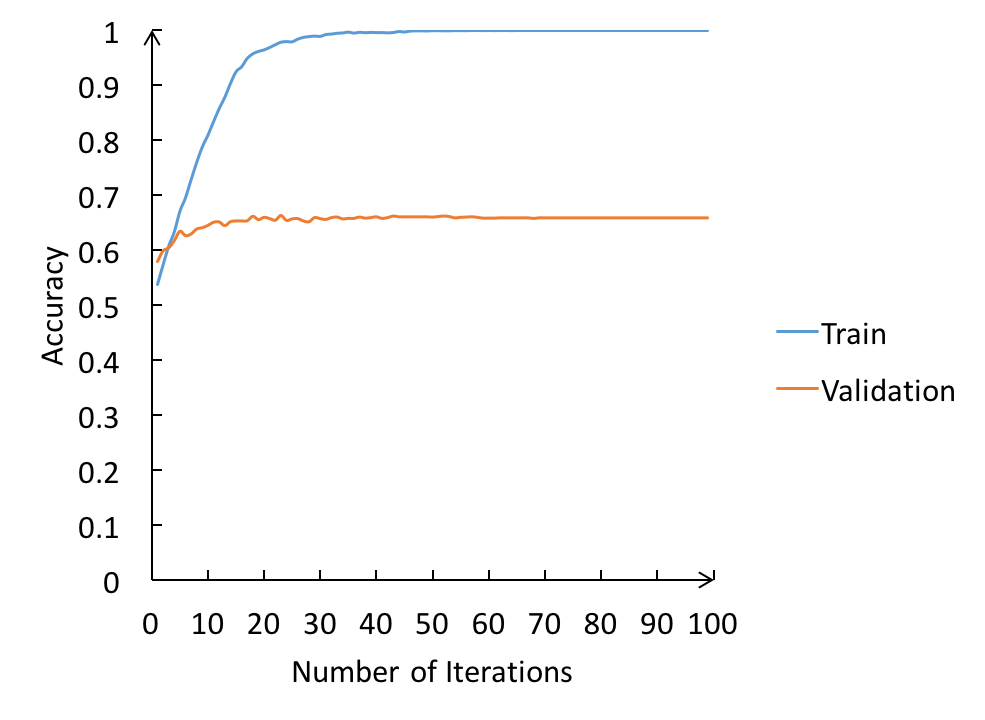
\includegraphics[width=\linewidth]{winnow_both.png}
\caption{Both} \label{fig:2c}
\end{subfigure}
\caption{Results for Winnow Algorithm} \label{fig:2}
\end{figure}
\subsubsection{Comparisons}
We can first compare among different feature sets. From the results shown above, we know that using both unigram and bigram contribute a lot with less iterations to converge and relatively high accuracy in validation set, for both perceptron and winnow algorithm. And unigram feature set also works well in this task to obtain a weight showing higher accuracy for both algorithms. 

Then compare between perceptron and winnow algorithm, we can observe that perceptron always shows higher accuracy than winnow and it takes less iterations for perceptron to converge or reach the highest accuracy. 
\subsection{Conclusions and Future Work}
In this task, two onling learning algorithm, Perceptron and Winnow, were implemented. Experiments with feature set of unigram, bigram and both of them were conducted. Validation set was applied to tune the hyper-parameter, number of iterations, in this task. The perceptron implemented in this task was of primal representation, in the future, dual representation can be implemented to improve the performance of this algorithm.
%\nocite{*}
%\bibliographystyle{plainnat}
%\bibliography{all}

\end{document}
